%=================================================================
% This template is based on IMRT Latex template by Eric A. Mueller
%================================================================= 

\documentclass[10pt,twoside,a4paper]{report}
 \usepackage[mt,hs,english]{ethasl}   % New styles and commands
                                      % Options: 	bt/mt: Bachelorthesis/Masterthesis
                                      %						fs/hs: Fr�hlingssemester/Herbstsemester
                                      %						german/english: Deutsch/English

% \includeonly{}                      % Quick formatting
% \usepackage[draft]{graphicx}        % Quick formatting

 \usepackage{a4}                      % Paper size
 \usepackage[latin1]{inputenc}        % Keybord settings
 \usepackage{amsmath}                 % Additional math functionality
 \usepackage{amssymb}                 % Additional math functionality
 \usepackage{graphicx}                % EPS figures
 \usepackage[dvips]{epsfig}           % EPS figures
 \usepackage{float}                   % Placement of floating objects
 \usepackage{fancyhdr}                % Headings
 \usepackage{rotating}
 \usepackage{multirow}
 \usepackage{url}
 \usepackage{colortbl}
 \usepackage{ifpdf}
 \usepackage{subfigure}



 \usepackage{hyperref}
 \usepackage{color}

 \usepackage[framed,numbered,autolinebreaks,useliterate]{mcode}
 \definecolor{black}{rgb}{0,0,0}
 \definecolor{white}{rgb}{1,1,1}

 \definecolor{darkred}{rgb}{0.5,0,0}
 \definecolor{darkgreen}{rgb}{0,0.5,0}
 \definecolor{darkblue}{rgb}{0,0,0.5}
 %\definecolor{zebg}{rgb}{1,1,.8} %elfenbeinfarbig
 
 \hypersetup{colorlinks
	,linkcolor=black
	,filecolor=black
	,urlcolor=black
	,citecolor=black
 }


\ifpdf
\usepackage[update]{epstopdf}
\else
\fi
% *** GRAPHICS RELATED PACKAGES ***
%

%\usepackage[pdftex]{graphicx}

%%%%%%%%%%%%%%
% My commands
%%%%%%%%%%%%%%
\newcommand{\figref}[1]{Fig. \ref{#1}}
\newcommand{\secref}[1]{Section \ref{#1}}
\newcommand{\neweulm}{\mbox{Neweul-M$^2$}}
\newcommand{\proneu}{\textit{pro}NEu}

% \usepackage{german}                  % German language
% \usepackage{ae}                      % German specials

%---------------------------------------------------------------------------

 \setlength{\parindent}{0em}                   % Disable parindent
 \rhead[\thepage]{\nouppercase{\rightmark}}    % Special headings
 \lhead[\nouppercase{\leftmark}]{\thepage}     % Special headings
 \cfoot{}                                      % Special headings

%---------------------------------------------------------------------------

 \title{proNEu Documentation}
 \headtitle{MATLAB Tool}
 \subtitle{Derivation of Analytical \\ \textbf{Kinematics} \& \textbf{Dynamics}}
 \keywords{dynamics, global kinematics, analytical equations of motion, projected Newton-Euler, simple MATLAB tool}
 \datepub{v1.1, Mar. 2012}
 \studentA{Marco Hutter}
 \studentB{Christian Gehring}
% \studentC{Student 3}
 
 

%\supervisionA{Andreas Muster}
%\supervisionB{Supervisor B}
%\supervisionC{Supervisor C}
 

%===========================================================================
\begin{document}

%---------------------------------------------------------------------------
% Title page

 \maketitle
 \pagestyle{plain}
 \pagenumbering{roman}

%---------------------------------------------------------------------------
% Preamble

 %---------------------------------------------------------------------------
% Preface

%\chapter*{Vorwort}

%Bla bla \dots

 %\cleardoublepage

%---------------------------------------------------------------------------
% Table of contents

% \setcounter{tocdepth}{2}
% \tableofcontents

%\cleardoublepage

%---------------------------------------------------------------------------
% Abstract

%\chapter*{Zusammenfassung}
% \addcontentsline{toc}{chapter}{Zusammenfassung}

%Bla bla \dots

% \cleardoublepage

\chapter*{Preamble}
 \addcontentsline{toc}{chapter}{Preamble}


This is the manual for the (very simple, but still quite powerfull) Matlab tool \proneu.  The tool uses the MATLAB Symbolic Math Toolbox\footnote{http://www.mathworks.ch/products/symbolic/} to derive the analytical global kinematics and equations of motion based on projected Newton-Euler methods.  In \secref{sec:theory}, a short summary about the theory (kinematics and dynamics) is given in combination with an outline of the implementation in MATLAB. \\ 
\begin{figure}[H]
	\centering
		\subfigure[3-link robot arm]{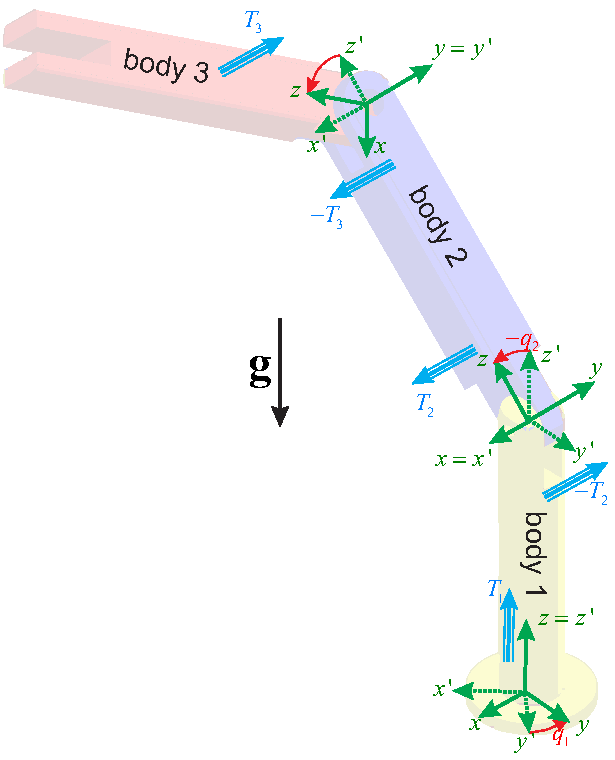
\includegraphics[height=3.5cm]{../RobotArmExample/robotArm3link_asm.pdf}}
		\subfigure[prismatic joint]{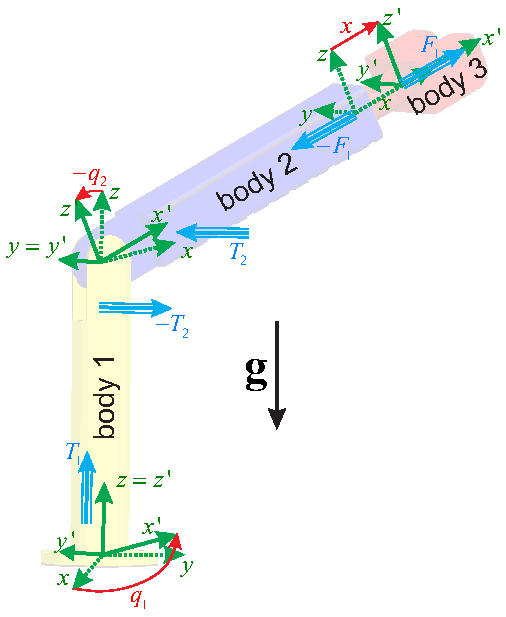
\includegraphics[height=3.5cm]{../RobotArmExample/robotArm_asm.pdf}}
		\subfigure[quadruped robot]{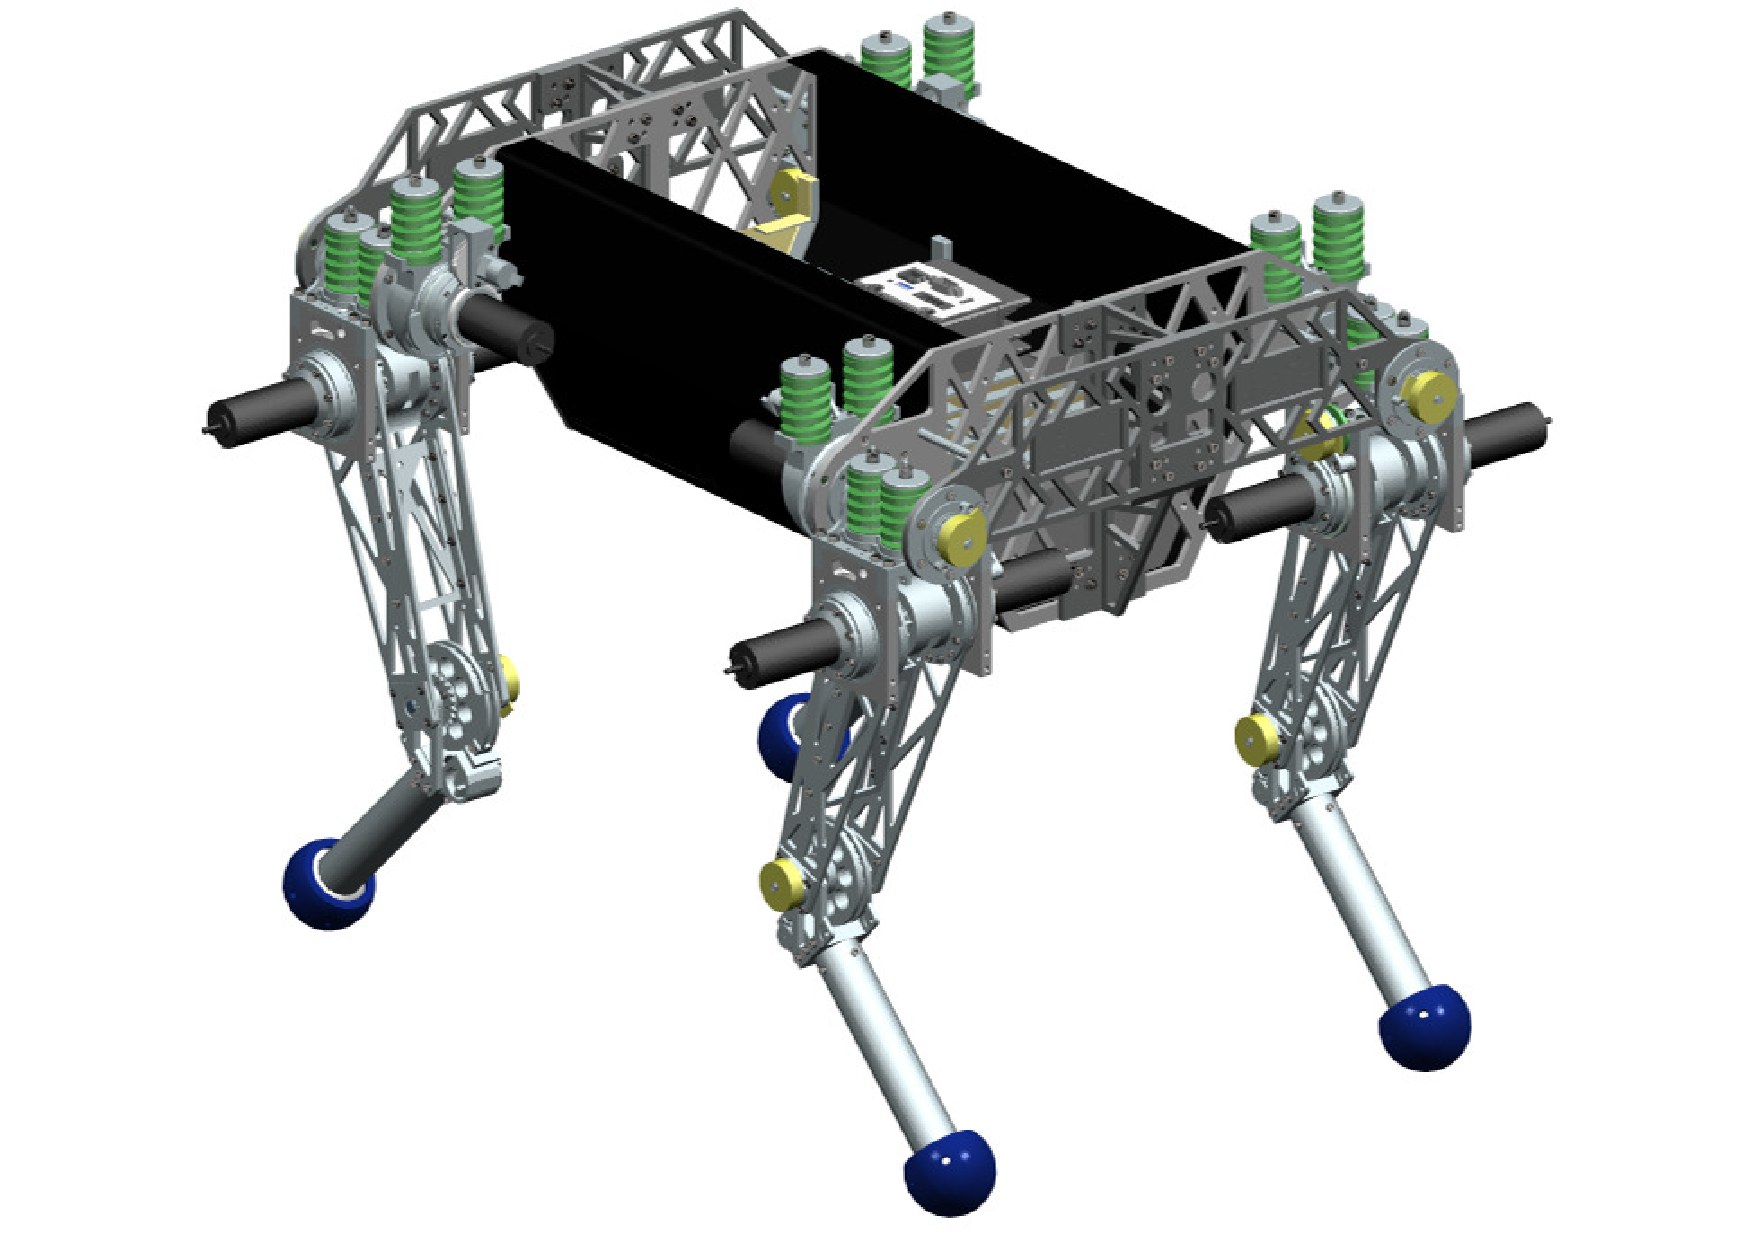
\includegraphics[height=3.5cm]{pics/3D_PR.pdf}}
	\caption{Three examples illustrating the use of this toolbox (\secref{sec:ex}).}
	\label{fig:exCol}
\end{figure}


Several examples (documented in \secref{sec:ex} as well as in the source files) highlight how this tool has to be used.  The user chooses the generalized coordinates, actuator and link parameters before setting up a very simple kinematic tree of the entire system.  The global kinematics and the equations of motion are symbolically derived and the user can visually check the robot configuration.  In the examples it is outlined, how the user can finally get function files, compiled mex-function, or C-code that can be used or embedded in any simulation environment.
\\

We intentionally kept this tool very simple for several reasons:  First, there exist (often commercially available) complex tools that are often a large overkill for most applications.  We do not want to have a sophisticated user front-end that allows adjusting everything without seeing behind the scenes, instead we appreciate tools where we can adapt everything for our needs.  In our specific case, we use this tool mostly for model based controllers, where we require to get the dynamics fast and efficiently in simulations or on the actual hardware.


\clearpage
% Version table
\begin{table}
\begin{tabular}[width=1\textwidth]{|p{2cm} p{10cm}|}
\hline
date: &Mar. 2012 \\
authors: &Christian Gehring \\
version: & 1.1 \\
info:    & minor fixes and improvements of the documentation, changed color of coordinate systems and added a world frame to plotBodies() \\
\hline
date: &Dec. 2011 \\
authors: &Marco Hutter \\
         &Christian Gehring \\
version: & 1.0 \\
info:    & First appearance of \proneu\\
\hline
\end{tabular}
\label{tab:version}
\caption{Revisions}
\end{table}


% software content table

\begin{table}
\begin{tabular}[width=1\textwidth]{|p{6cm} p{7cm}|}
\hline
\footnotesize \bf{utils/} &\footnotesize utility folder\\
\footnotesize.../computePNE.m & \footnotesize core file for global dynamics and projected Newton-Euler equations\\
\footnotesize.../dMATdt.m & \footnotesize full differentiation \\
\footnotesize.../eulerToRotMat$\_$A$\_$IB.m &\footnotesize rotation matrix from B to I frame, x-y-z definition \\
\footnotesize.../eulerToRotMat$\_$A$\_$BI.m &\footnotesize rotation matrix from I to B frame, x-y-z definition \\
\footnotesize.../plotBodies.m &\footnotesize visualization of (global) kinematic tree \\
\footnotesize.../skew.m &\footnotesize get skewing a matrix from vector \\
\footnotesize.../unskew.m &\footnotesize skew matrix to vector \\
\hline
\footnotesize\bf{examples/} &\footnotesize example folder\\
\footnotesize.../QuadrupedFreeFloat/genEoM.m &\footnotesize free floating quadruped Starl\textit{ETH} \\
\footnotesize.../RA3Link/genEoM.m &\footnotesize robot arm with 3 links and 3 revolute joints\\
\footnotesize.../RA3LinkPrismatic/genEoM.m &\footnotesize robot arm with 3 links and 1 prismatic joint \\
\footnotesize.../GenerateCode/createFunctionFiles.m &\footnotesize generating matlab and functions \\
\footnotesize.../GenerateCode/genCCodeMatrix.m &\footnotesize generate c-code of marix function \\
\footnotesize.../GenerateCode/genCCodeVariables.m &\footnotesize define parameters for c-code \\
\footnotesize.../GenerateCode/genCCodeExampleFile.m &\footnotesize example for c-code \\
\hline
\end{tabular}
\label{tab:content}
\caption{Software file content}
\end{table}
\normalsize
 \cleardoublepage

%---------------------------------------------------------------------------

% Table of contents

 \setcounter{tocdepth}{2}
 \tableofcontents
 
 \cleardoublepage

 \pagestyle{headings}                 % Default headings
 \pagestyle{fancy}                   % Special headings
 \pagenumbering{arabic}

%---------------------------------------------------------------------------
% Chapters
%\input{sections/introduction}
\chapter{Theoretical Background and Notation}\label{sec:theory}

\section{Kinematics}\label{sec:kinematics}
This section gives a compact overview about the notation for the kinematic and dynamic representation.  Each part is accompanied by some code snippets that should highlight how this works in Matlab.  Note: these code parts DO NOT belong to a specific example.  For complete examples check \secref{sec:ex}.

\subsection{Generalized Coordinates}
We use generalized coordinates $\mathbf{q}$ that can contain in the case of free floating bodies in addition to the joint coordinates $\mathbf{q}_{r}$ also un-actuated base coordinates $\mathbf{q}_b$: 
\begin{equation}
\mathbf{q} = \left( \begin{array}{c} \mathbf{q}_{b} \\ \mathbf{q}_{r} \end{array}\right).
\end{equation}

\begin{lstlisting}
% define generalized coordinates 
syms x q1 q2 real
q = [x,q1,q2]';
% define generalized velocities
syms Dx Dq1 Dq2 real
dq = [Dx,Dq1,Dq2]';
\end{lstlisting}

\subsection{Position Vector}
A (position) vector from point $O$ to $P$ as a function of generalized coordinates $\mathbf{q}$ expressed in frame $B$:
\begin{equation}
_B \mathbf{r}_{OP} = _B \mathbf{r}_{OP}\left(\mathbf{q}\right).
\end{equation}
\begin{lstlisting}
% define certain parameters
syms l real
% position vector
r = [l*sin(q1),l*cos(q1),0];
\end{lstlisting}


\subsection{Velocity (in Moved Systems)}\label{sec:velocity}
The velocity is given through differentiation, whereby special attention is required when differentiating in a moving (with respect to inertial frame $I$) coordinates system $B$:
\begin{eqnarray}
_I\mathbf{r} \rightarrow {}_I\dot{\mathbf{r}} &=& \frac{d{}_I\mathbf{r}}{dt} \\
_B\mathbf{r} \rightarrow {}_B\dot{\mathbf{r}} &=& \frac{d{}_B\mathbf{r}}{dt} + _B\omega_{IB} \times _B\mathbf{r}
\end{eqnarray}
In this document, $O$ refers to the origin of a frame, $I$ indicates the inertial frame and $B$ a body fixed frame (which can be moved).
\\

%In the special case of rigid body kinematics we introduce the body rotation speed $\boldsymbol{\Omega}$
%\begin{equation}
%\boldsymbol{\Omega} = {}_I\omega_{IB}
%\end{equation}


\begin{lstlisting}
% derivation of position vectors expressed in inertia frame
dr = dMATdt(r,q,dq);
\end{lstlisting}

\subsection{Rotation}
\begin{figure}[H]
	\centering
		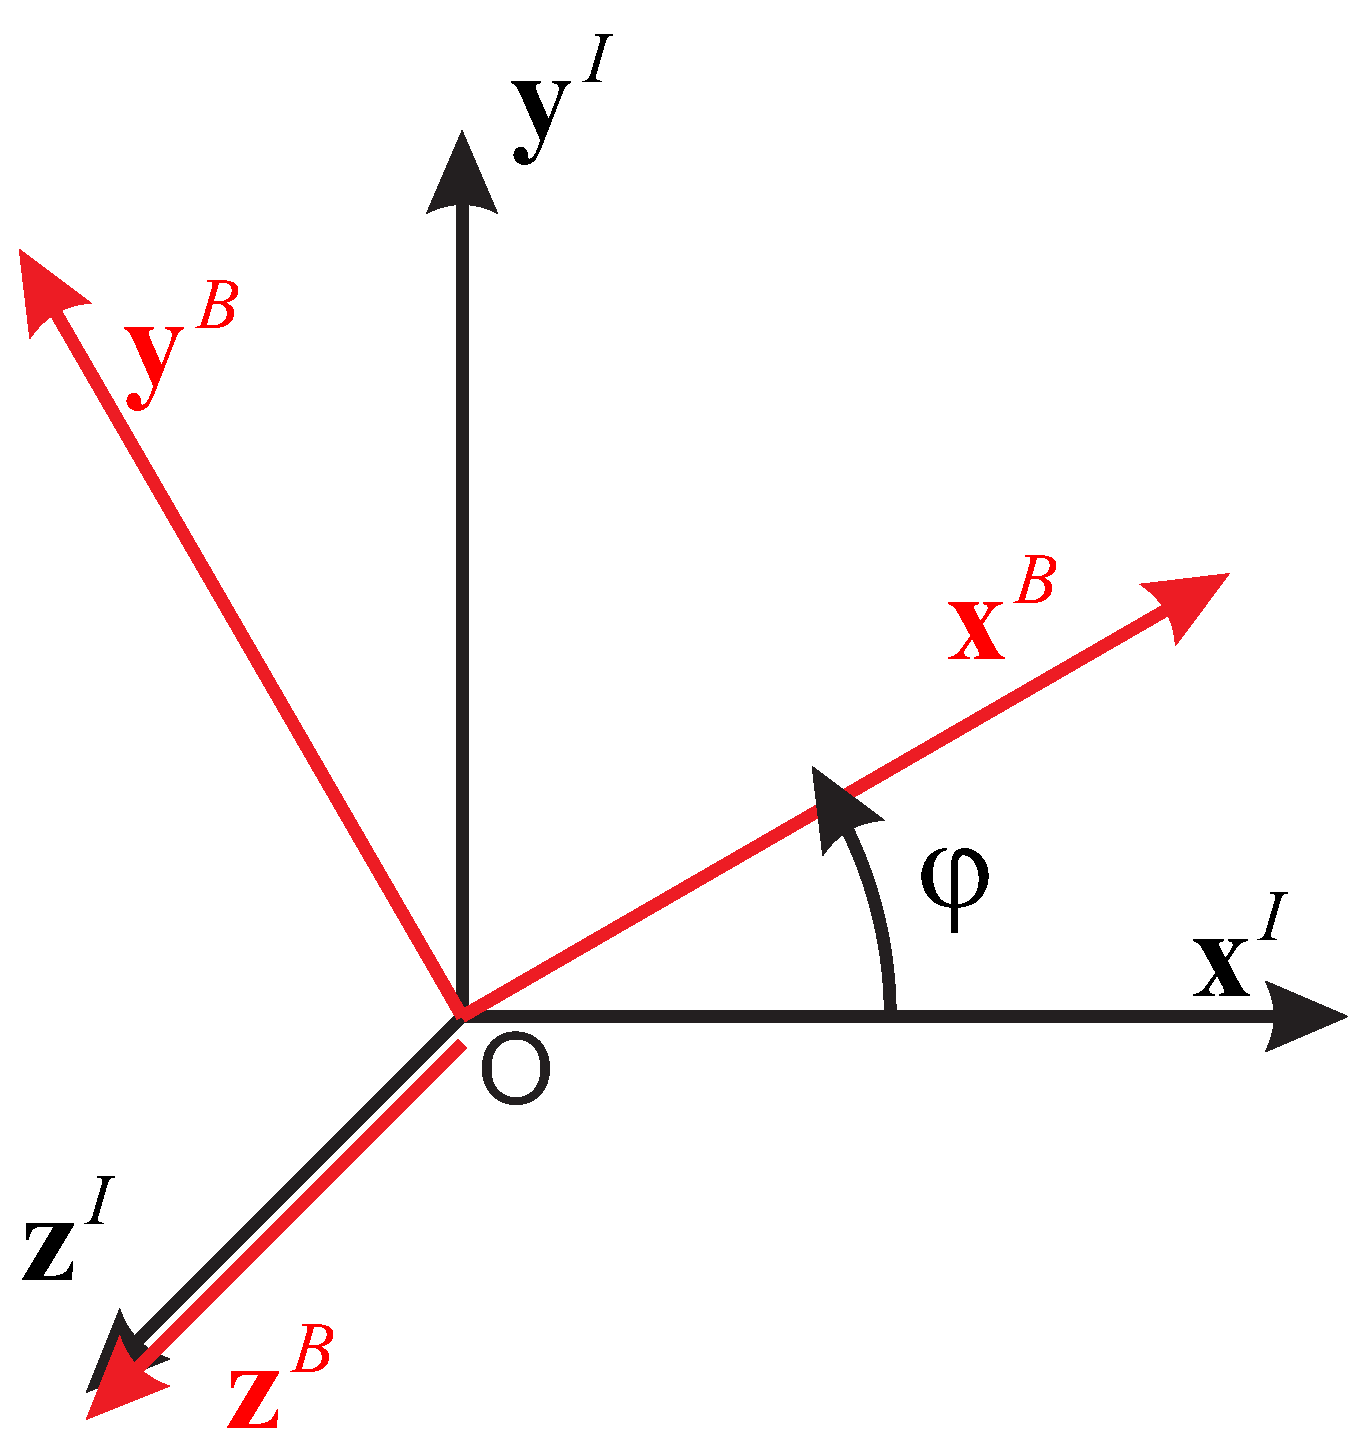
\includegraphics[width=.500\textwidth]{pics/movedCS.pdf}
	\caption{Rotated coordinate system $B$ around z axis}
	\label{fig:movedCS}
\end{figure}

The rotation matrix $\mathbf{A}_{IB}$ rotates a vector $_B\mathbf{r}$ expressed in frame $B$ to frame $I$:
\begin{eqnarray}
_I\mathbf{r} &=& \mathbf{A}_{IB} {}_B\mathbf{r}\\
_B\mathbf{r} &=& \mathbf{A}_{BI} {}_I\mathbf{r} \qquad \mathbf{A}_{BI} = \mathbf{A}_{IB}^T\\
_C\mathbf{r} &=& \mathbf{A}_{CI} {}_I\mathbf{r} \qquad \mathbf{A}_{CI} = \mathbf{A}_{CB}\mathbf{A}_{BI}
\end{eqnarray}

In this tool we use the x-y-z convention (see MATLAB code below).

\begin{lstlisting}
% rotation matrix around z with angle phi [rad]
syms phi real
AIB = eulerToRotMat_A_IB(0,0,phi);
% Note: we use here the x-y-z definition, so the rotation matrix with angles alpha, beta and gamma 
syms alpha beta gamma real
AIB = eulerToRotMat_A_IB(alpha,beta,gamma);
% is equivalent to
AIB = eulerToRotMat_A_IB(alpha,0,0)*...  		% rot around x 
			eulerToRotMat_A_IB(0,beta,0)*... 		% rot around y
			eulerToRotMat_A_IB(0,0,gamma); 			% rot around z
\end{lstlisting}

More details can be found in the matlab function files:
\begin{itemize}
\item /utils/eulerToRotMat\_A\_IB.m 
\item /utils/eulerToRotMat\_A\_BI.m.
\end{itemize}


\subsection{Angular Velocity}
Given a rotation matrix $\mathbf{A}_{IB}$, the corresponding rotation speed $_I\boldsymbol{\Omega}$ of a rigid body with body fixed frame $B$ is:
\begin{eqnarray}
_I\tilde{\boldsymbol{\Omega}} &=& {}_I\tilde{\boldsymbol{\omega}}_{IB} = \dot{\mathbf{A}}_{IB}\mathbf{A}_{IB}^T \\
\tilde{\boldsymbol{\Omega}} &=& \left[\begin{array}{ccc} 0&-\Omega^z & \Omega^y \\ \Omega^z & 0 & -\Omega^x \\ -\Omega^y & \Omega^x & 0\end{array}\right],\quad \begin{array}{c} unskew \\ \rightleftharpoons \\ skew \end{array} \quad \boldsymbol{\Omega} = \left(\begin{array}{c} \Omega^x\\ \Omega^y\\ \Omega^z \end{array} \right)
\end{eqnarray} 

\begin{lstlisting}
% rotation matrix around z with vector phi
AIB = eulerToRotMat_A_IB(0,0,phi);
% differentiate rotation matrix
dAIB = dMATdt(AIB,q,dq);
% generate rotation speed and unskew it
I_Omega = unskew(simplify(dAIB*AIB'));
\end{lstlisting}


\subsection{Jacobian}\label{sec:jacobian}
The Jacobian $\mathbf{J}$ is given through:
\begin{equation}
\mathbf{J}\left(\mathbf{q}\right) = \frac{\partial \mathbf{r}\left(\mathbf{q}\right)}{\partial\mathbf{q}} = 
\left[
\begin{array}{cccc}
\frac{\partial\mathbf{r}_1}{\partial\mathbf{q}_1} & \frac{\partial\mathbf{r}_1}{\partial\mathbf{q}_2} & \ldots & \frac{\partial\mathbf{r}_1}{\partial\mathbf{q}_n} \\
\frac{\partial\mathbf{r}_2}{\partial\mathbf{q}_1} & \frac{\partial\mathbf{r}_2}{\partial\mathbf{q}_2} & \ldots & \frac{\partial\mathbf{r}_2}{\partial\mathbf{q}_n} \\
\vdots & \vdots & \ddots & \vdots \\
\frac{\partial\mathbf{r}_m}{\partial\mathbf{q}_1} & \frac{\partial\mathbf{r}_m}{\partial\mathbf{q}_2} & \ldots & \frac{\partial\mathbf{r}_m}{\partial\mathbf{q}_n}
\end{array}
\right], 
\qquad {\mathbf{q}}\in \Re^{n\times1}, \mathbf{r}\in\Re^{m\times1}
\end{equation}
Jacobians are used to map generalized velocities $\dot{\mathbf{q}}$ to Cartesian velocities $\dot{\mathbf{r}}$: 
\begin{equation}
\dot{\mathbf{r}} = \mathbf{J}\dot{\mathbf{q}}
\end{equation}
and in its dual problem to map Cartesian forces $\mathbf{F}$ to generalized forces $\boldsymbol{\tau}$:
\begin{equation}
\boldsymbol{\tau} = \mathbf{J}^T\mathbf{F}
\end{equation}

We differ between translational Jacobians $\mathbf{J}_{P} = \frac{\partial \mathbf{r}_{P}\left(\mathbf{q}\right)}{\partial \mathbf{q}}$, which correspond to a specific point $P$ and rotational Jacobians $\mathbf{J}_{R} = \frac{\partial \boldsymbol{\Omega}\left(\mathbf{q}\right)}{\partial \dot{\mathbf{q}}}$ that are identical for all points of one single rigid body.

\begin{lstlisting}
% get jacobian from position vector
J = jacobian(r,q);
% get jacobian from rotation speed
Jr = jacobian(Omega,dq); 
\end{lstlisting}


%%%%%%%%%%%%%%%%%%%%%%%%%%%%%%%%%%%%%%%%%%%%%%%%%%%%%%%%%%%%%%%%%%%%%%%
\clearpage
\section{Dynamics}
The goal of this tool is to get the equations of motion in the following form
\begin{equation}\label{eq:eom}
\mathbf{M}\left(\mathbf{q}\right) \ddot{\mathbf{q}} + \mathbf{b}\left(\mathbf{q},\dot{\mathbf{q}}\right) + \mathbf{g}\left(\mathbf{q}\right) = \mathbf{S}^T \boldsymbol{\tau}
\end{equation}
with 
\\

\begin{tabular}{ll}
$\mathbf{M}$: & mass matrix $\in \Re^{n\times n}$\\
$\mathbf{b}$: & coriolis and centrifugal components $\in \Re^{n\times 1}$\\
$\mathbf{g}$: & gravitational components $\in \Re^{n\times 1}$\\
$\mathbf{S}^T$: & selection matrix of the actuated joints $\in \Re^{k\times n}$\\
$\boldsymbol{\tau}$: & generalized forces $\in \Re^{k\times 1}$ \\
$n$: & number of degrees of freedom \\
$k\leq n$: & number of actuated joints
\end{tabular} 
\\
\textit{Note:} This tool is written for the most common type of systems. All bindings are skleronomic (time independent) and holonomic.  Algebraic differential equations (ADE) are not supported.

\subsection{Projected Newton-Euler Equations}
This framework is based on projected Newton-Euler equations, which can be understood as projection of the conservation of impulse $\mathbf{p}$ and angular momentum $\mathbf{N}_S$ onto generalized coordinates:
\begin{equation}
\sum_{i=1}^N{\mathbf{J}_{S_i}^T \dot{\mathbf{p}}_i + \mathbf{J}_{R_i}^T \dot{\mathbf{N}}_{S_i} - \mathbf{J}_{S_i}^T\mathbf{F}^a_{S_i}} - \mathbf{J}_{R_i}^T\mathbf{T}^a_i = \mathbf{0}
\end{equation}

\begin{eqnarray}
\mathbf{p}_i\left(\mathbf{q}\right) = m_i\dot{\mathbf{r}}_{OS_i} && \text{impulse} \\
\mathbf{N}_{S_i} = \boldsymbol{\theta}_{S_i}\mathbf{\Omega}_i && \text{angular momentum} \\
\mathbf{F}^a_{S_i} && \text{external forces} \\
\mathbf{T}^a_i && \text{external torques}
\end{eqnarray}
with $S_i$ correspoding to the Center of Gravity of link $i$.  Knowing that the change of impulse and angular momentum can be written as 
\begin{eqnarray}
\dot{\mathbf{p}}_i = m_i \ddot{\mathbf{r}}_{OS_i} \\
\dot{\mathbf{N}}_{S_i} = \boldsymbol{\theta}_{S_i} \dot{\boldsymbol{\Omega}}_i + \boldsymbol{\Omega}_i\times\boldsymbol{\theta}_{S_i}\boldsymbol{\Omega}_i
\end{eqnarray}
where $\boldsymbol{\theta}_{S_i}\in \Re^{3\times 3}$ is the inertia of body $i$ w.r.t. the Center of Gravity.  Using the kinematic relations
\begin{eqnarray}
\ddot{\mathbf{r}}_{OS_i} &=& \mathbf{J}_{S_i}\ddot{\mathbf{q}}+\dot{\mathbf{J}}_{S_i}\dot{\mathbf{q}} \\
\boldsymbol{\Omega}_i &=& \mathbf{J}_{R_i} \dot{\mathbf{q}} \\
\dot{\boldsymbol{\Omega}}_i &=& \mathbf{J}_{R_i} \ddot{\mathbf{q}} + \dot{\mathbf{J}}_{R_i} \dot{\mathbf{q}}
\end{eqnarray}
the elements of \eqref{eq:eom} are obtained by
\begin{eqnarray}
\mathbf{M}\left(\mathbf{q}\right) &=& \sum_{i=1}^N{\mathbf{J}_{S_i}^T m_i\mathbf{J}_{S_i} + \mathbf{J}_{R_i}^T \boldsymbol{\theta}_{S_i} \mathbf{J}_{R_i}}\\
\mathbf{b}\left(\mathbf{q}\right) &=& \sum_{i=1}^N{\mathbf{J}_{S_i}^T m_i\dot{\mathbf{J}}_{S_i}\dot{\mathbf{q}}+
\mathbf{J}_{R_i}^T \boldsymbol{\theta}_S \dot{\mathbf{J}}_{R_i}\dot{\mathbf{q}} + \boldsymbol{\Omega}_i\times\boldsymbol{\theta}_{S_i}\boldsymbol{\Omega}}_i \\
\mathbf{g}\left(\mathbf{q}\right) &=& \sum_{i=1}^N{-\mathbf{J}_{S_i}^T\mathbf{F}_{S_i}^g}
\end{eqnarray} 

\cleardoublepage
\chapter{Matlab Tool}

The presented tool uses the Symbolic Math Toolbox\footnote{http://www.mathworks.ch/products/symbolic/}. 

\section{Kinematic Tree}\label{sec:kintree}
The robot is described as a kinematic tree.  
A root element needs to be selected first and from there the individual branches are successively described.
Each rigid body has to be described with the following struct:


\begin{lstlisting}
% => start setting up the kinematic structure.  Each link needs to have all the folowing struct elements 
% B indicates bodyframe
% P indicates coordinate system of parent element

% body(i).param.m: 			 body mass
% body(i).param.B_Th: 	 inertia tensor in body frame w.r.t. CoG
% body(i).param.B_r_COG: CoG in body frame
% body(i).cs.P_r_PO:		 position of origin in parent CS
% body(i).cs.A_PB:  		 rotation from parent CS
% body(i).tree.parent:   tree parent (0=inertial frame)

%% Body 1
i = 1;
% body mass
body(i).param.m = m1;   
body(i).param.B_Th = diag([Th1_xx Th1_yy Th1_zz]); 
body(i).param.B_r_COG = [0;0;s1];
body(i).cs.P_r_PO = sym([0;0;0]); % ensure a symbolic expression
body(i).cs.A_PB = eulerToRotMat_A_IB(0,0,q1);
body(i).tree.parent = 0;
\end{lstlisting}
Some notes on the notation:\\
\begin{tabular}{ll}
$_B\boldsymbol{\theta}$: & Inertia of the body with respect to CoG expressed in body fixed frame B\\
$_B\mathbf{r}_{CoG}$: & Vector from origin of body fixed frame to CoG expressed in body frame B\\
$_P\mathbf{r}_{PO}$: & Translational vector from origin of parent frame P \\ & to origin of body frame B expressed in parent frame P \\
$\mathbf{A}_{PB}$: & Rotation matrix that rotates a vector expressed in body frame B to parent frame P
\end{tabular}
See Figure~\ref{fig:3D_PR}, which represents a 3-link robot arm, to better understand the definition of the vectors.
\clearpage
\section{Force Elements}\label{sec:forceel}
This framework allows to describe both force (prismatic, type = 'lin') and torque (rotational, type='rot') actuators.  

\begin{figure}[H]
	\centering
		\subfigure[Torque actuator acting in a revolute joint (type = 'rot').]{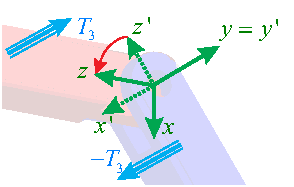
\includegraphics[width=0.3\textwidth]{../RobotArmExample/revoluteJoint.pdf}}\qquad\qquad
		\subfigure[Force actuator acting in a prismatic joint (type = 'lin').]{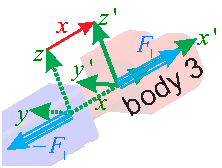
\includegraphics[width=0.3\textwidth]{../RobotArmExample/linearJoint.pdf}}
		%\subfigure[Torque actuator acting in a revolute joint (type = 'rot').]{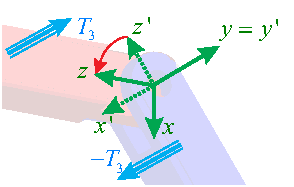
\includegraphics[width=0.3\textwidth]{../RobotArmExample/revoluteJoint.pdf}}\qquad\qquad
		%\subfigure[Force actuator acting in a prismatic joint (type = 'lin').]{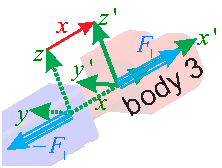
\includegraphics[width=0.3\textwidth]{../RobotArmExample/linearJoint.pdf}}
	\caption{Two types of force elements can be defined.}
	\label{fig:joints}
\end{figure}

\subsection{Torque Actuators} \label{sec:torqueAct}

This is the most common actuator for all types of robotic arms.  They are defined as follows:
\begin{lstlisting}
% torque element acting between environment and body 1
i = 1;
ftel(i).type = 'rot';       % define it to be a rotational = torque 
ftel(i).body_P = 0;         % body on which the reaction happens
ftel(i).body_B = 1;         % body on which the action happens
ftel(i).B_T = [0;0;T1];     % torque vector, expressed in B frame
\end{lstlisting}
For a detailed example, please check \secref{sec:3link}.

\subsection{Force Actuators}
Prismatic joints (like hydraulic/pneumatic cylinders, spindle drives, etc.) are defined as follows:
\begin{lstlisting}
% force element acting between body 2 and body 3
i = 3;
ftel(i).type = 'lin';        % define it to be a rotational = torque 
ftel(i).body_P = 2;          % body on which the reaction happens
ftel(i).body_B = 3;          % body on which the action happens
ftel(i).P_r_R = sym([0;0;0]);% point of reaction in P frame
ftel(i).B_r_A = sym([0;0;0]);% point of action in B frame
ftel(i).B_F = [F1;0;0];      % force vector of action 
\end{lstlisting}
For a detailed example, please check \secref{sec:3linkPris}.

\textit{Note:} The case of a cylinder attached to two bodies that are connected over a revolute joint falls (although being a linear actuator) into the category of torque actuators (\secref{sec:torqueAct}).  

\begin{figure}[H]
	\centering
		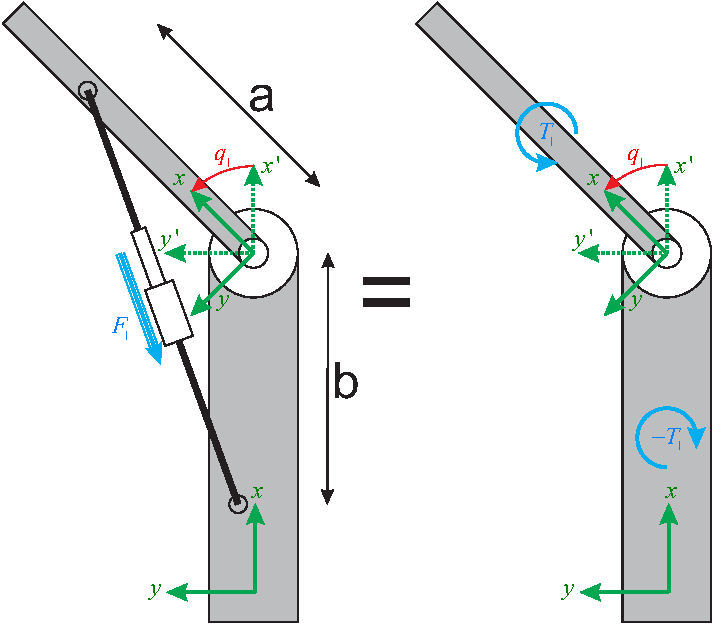
\includegraphics[width=0.6\textwidth]{../RobotArmExample/robotArm_cylinder.pdf}
	\caption{A cylinder in combination with a revolute joint has to be modeled as a torque actuator.}
	\label{fig:robotArmcylinder}
\end{figure}

The linear force $F_1$ with the two joint offsets $a,b$ can be transformed to a joint torque $T_1=f\left(q_1,a,b,F_1\right)$:
\begin{eqnarray}
\phi &=& \tan^{-1}\left(\frac{a\sin{q_1}}{b+a\cos{q_1}}\right) \\
T_1 &=& F_1 b\sin{\phi}
\end{eqnarray}


\section{Projected Newton-Euler Equations}
After the setup of the relative body kinematics (\secref{sec:kintree}) and the force elements (\secref{sec:forceel}) we can calculate the absolute kinematics and dynamics of the system by applying the projected Newton-Euler method:

\begin{lstlisting}
function [sys, body, ftel] = computePNE(body,ftel,q,dq,tau,I_a_grav)
 
% INPUT:
% * body:       kinematic tree
% * ftel:       force/torque elements
% * q:          generalized coordinates (symb) in desired order
% * Dq:         coresponding velocities
% * tau:        actuator force/torque array (symb)
% * I_a_grav:   gravity vector (R3)
%
% OUTPUT:
% * sys:        system struct containing dynamcis (all symbolic)
%   .MpNE:      mass matrix
%   .bpNE:      coriolis/centrifugal
%   .gpNE:      gravity terms
%   .SpNE:      actuator selection matrix
%   .fpNE:      =SpNE*T;
%   .param:     input parameters
%   .q:         generalized coordinates
%   .Dq:        generalized velocities
%   .tau        generalized actuator forces
%
% * body.kin:   body contains (among others) now also global kinematics as:
%   .A_IB:      rotation matrix from B to I (inertial/world frame)
%   .I_r_O:     vector inertial frame to body frame
%   .I_dr_O:    velocity of body frame in inertia frame
%   .I_r_CoG:   center of gravity position represented in inertia frame
%   .I_dr_CoG:  velcity ...
%   .I_J_CoG:   CoG jacobian
%   .I_Jr:      rotation jacobian
%   .I_Omega:   body rotational speed
%   ... and a lot more  

\end{lstlisting}



\cleardoublepage
\chapter{Examples}\label{sec:ex}
This is a collection of validated (with the software \neweulm \cite{kurz_neweul_2010}) examples: \\
\begin{tabular}{|l|l|}
\hline
Examples/RA3Link/ & 3-link robot arm (\secref{sec:3link}) \\ \hline
Examples/RA3LinkPrismatic/ & 3-link robot arm with prismatic joint (\secref{sec:3linkPris}) \\ \hline
Examples/QuadrupedFreeFloat/ & free floating quadruped (\secref{sec:quadruped}) \\ \hline
\end{tabular}

%%%%%%%%%%%%%%%%%%%%%%%%%%%%%%%%%%%%%%%%%%%%%%%%%%%%%%%%%%%%%%%%%%%%%%%%%%%%%%%%%%%%%%%%%%
\section{3-link Robot Arm} \label{sec:3link}
\begin{figure} [H]
	\centering
		\subfigure[3-link arm]{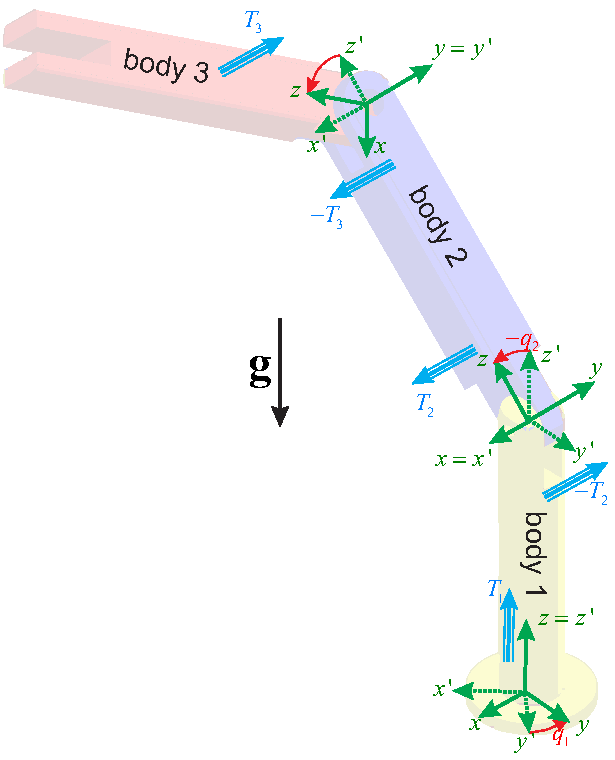
\includegraphics[width=0.4\textwidth]{../RobotArmExample/robotArm3link_asm.pdf}}\qquad
		\subfigure[Description of the second body]{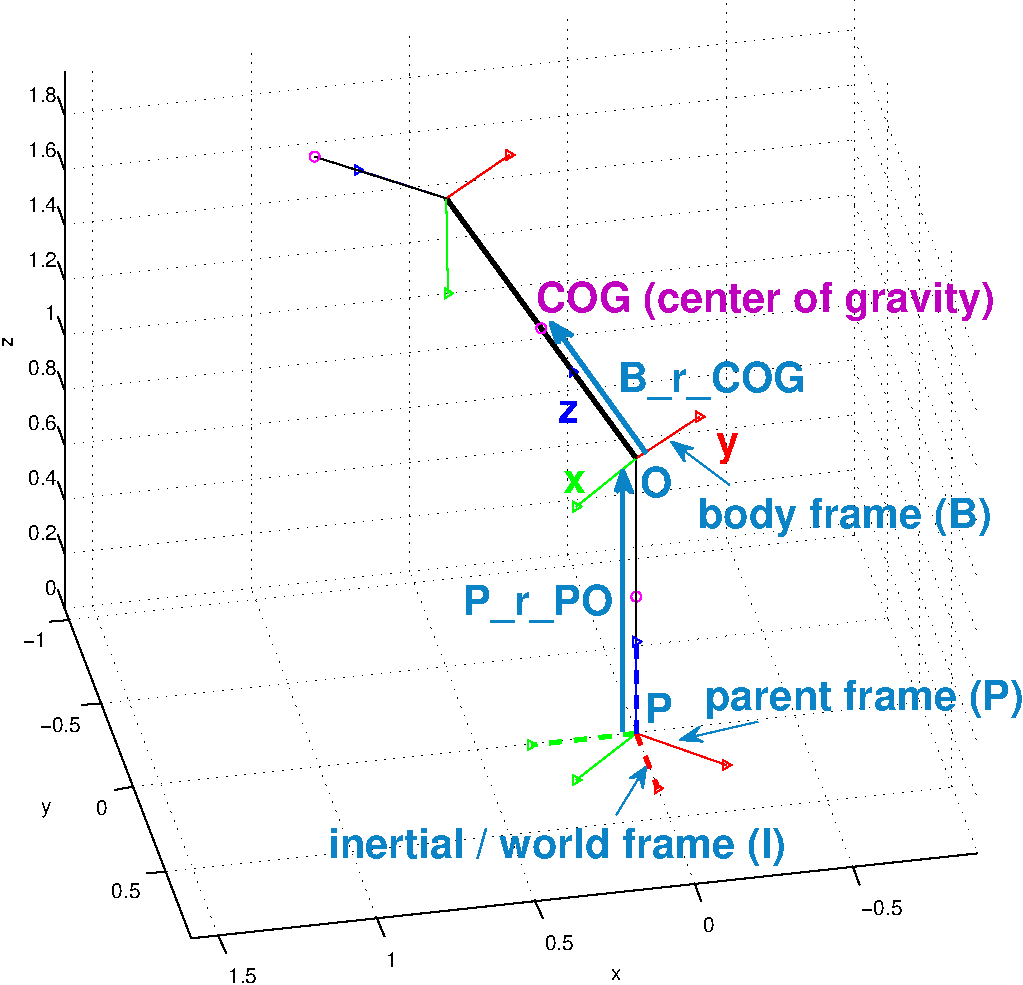
\includegraphics[width=0.5\textwidth]{../RobotArmExample/robotArm3link_plotBodies}}	
	\caption{3-link robot arm with three revolute joints ($\mathbf{z},\mathbf{x},\mathbf{y}$).}
	\label{fig:3D_PR}
\end{figure}

\lstinputlisting{../../examples/RA3Link/genEoM.m}

%%%%%%%%%%%%%%%%%%%%%%%%%%%%%%%%%%%%%%%%%%%%%%%%%%%%%%%%%%%%%%%%%%%%%%%%%%%%%%%%%%%%%%%%%%%%%
\clearpage
\section{3-link Robot Arm with Prismatic Joint} \label{sec:3linkPris}
\begin{figure}[H]
	\centering
		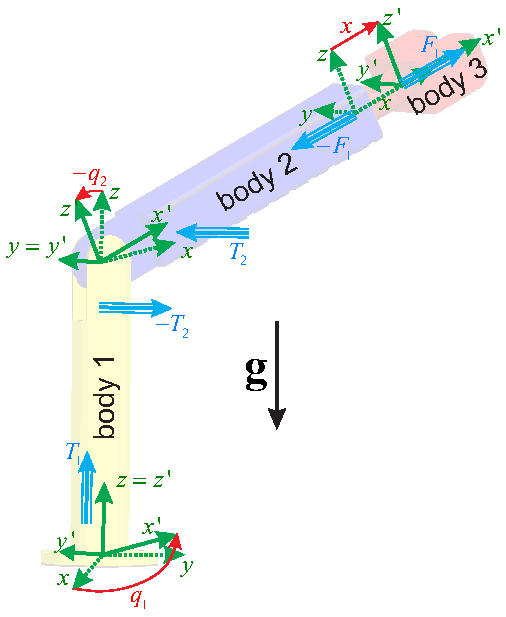
\includegraphics[width=0.50\textwidth]{../RobotArmExample/robotArm_asm.pdf}
	\caption{3-link robot arm with two revolute joints ($\mathbf{z},\mathbf{y}$) and one prismatic joint ($\mathbf{x}$).}
	\label{fig:robotArm_asm}
\end{figure}


\lstinputlisting{../../examples/RA3LinkPrismatic/genEoM.m}


%%%%%%%%%%%%%%%%%%%%%%%%%%%%%%%%%%%%%%%%%%%%%%%%%%%%%%%%%%%%%%%%%%%%%%%%%%%%%%%%%%%%%%%%%%%%%
\clearpage


\section{Quadruped Robot Starl\textit{ETH}}\label{sec:quadruped}
For detailed information about our quadruped Starl\textit{ETH} please consult our homepage\footnote{leggedrobotics.ethz.ch}.  Here is a brief outline: each leg has 3 degrees of freedom (x-rotation for hip abduction/adduction, followed by y-rotation for hip flexion/extension as well as y-rotation for knee flexion/extension) and is connected to a free floating main body.
\\
This model shows also how to model a free floating body as well as ground contact.  Adding dummy-bodies as feet allow to directly get the support Jacobians needed for modeling the hard ground contact (impact as well as contact constraints).
\begin{figure} [H]
	\centering
		\subfigure[]{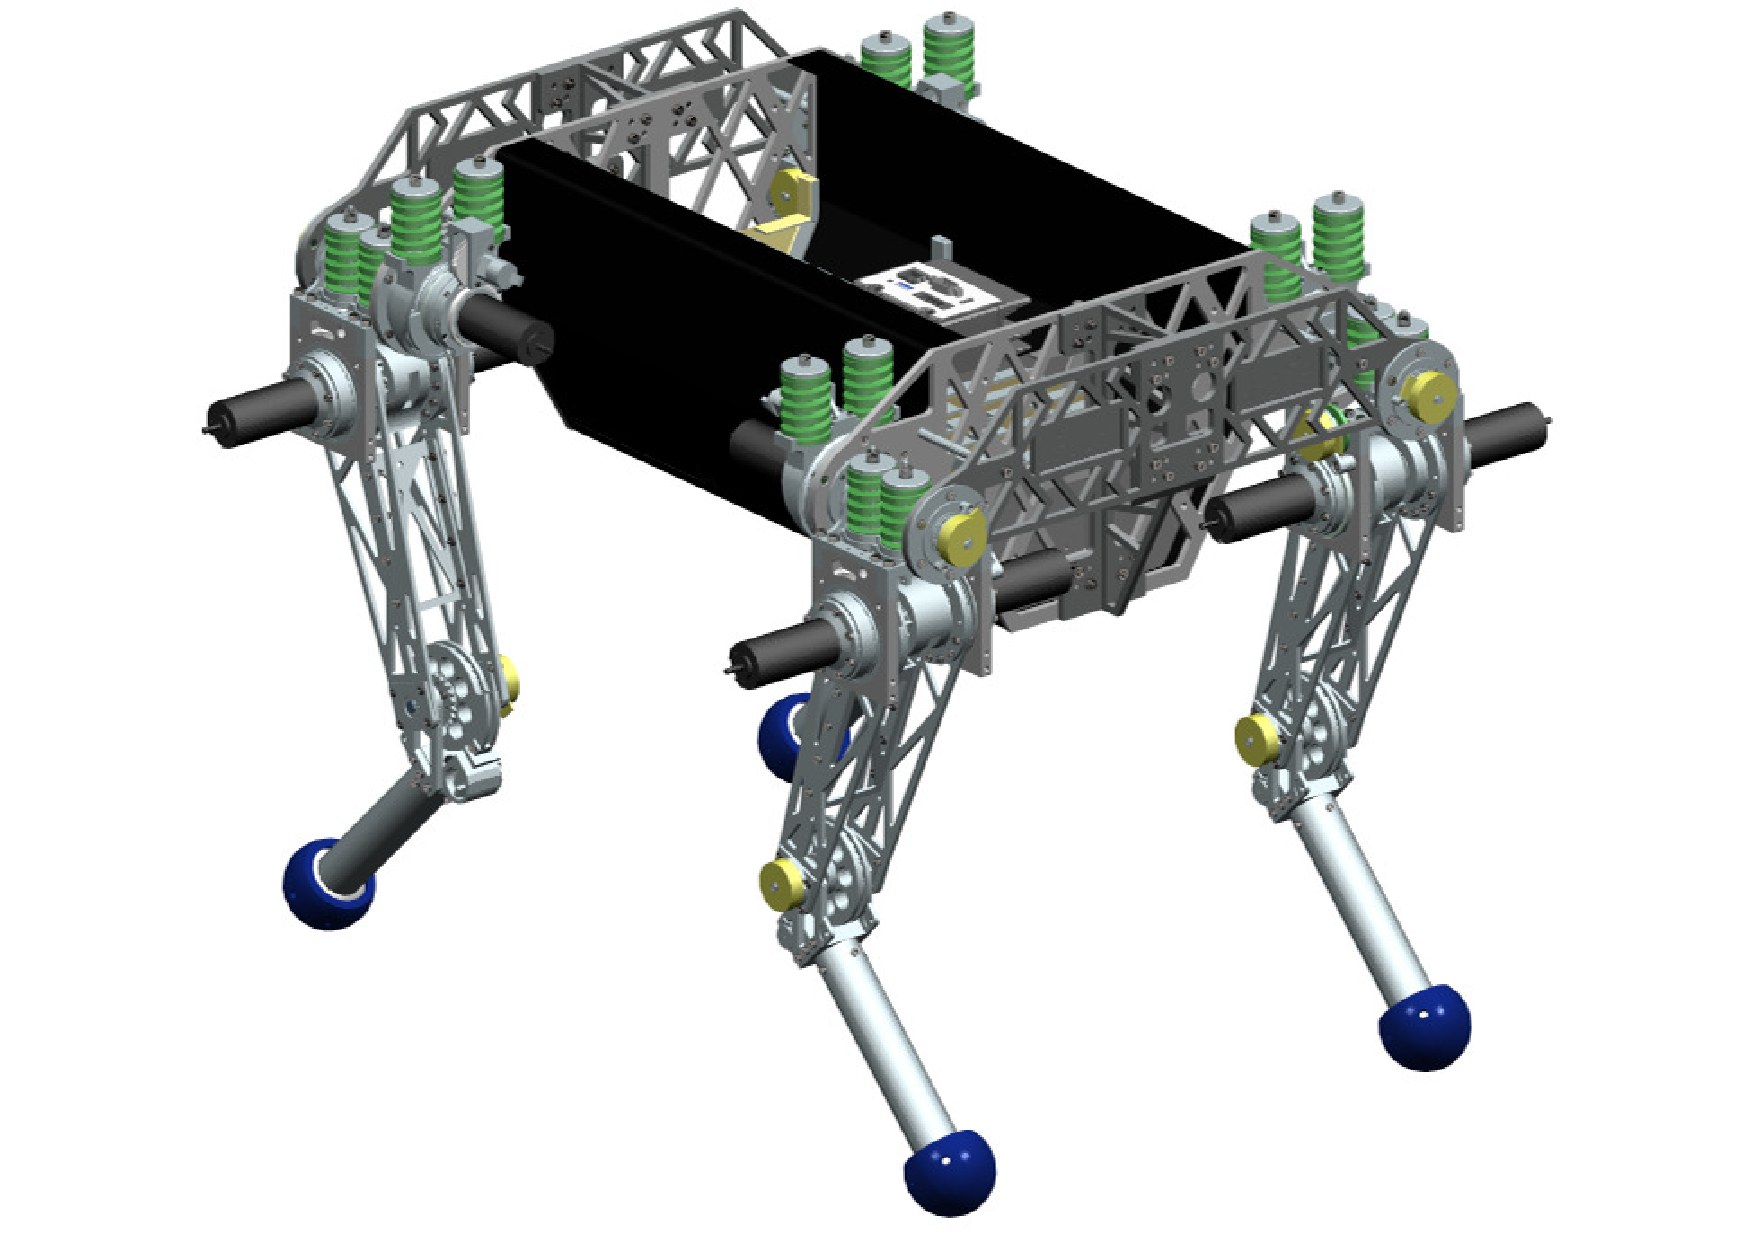
\includegraphics[width=0.5\textwidth]{pics/3D_PR.pdf}}\qquad
		\subfigure[]{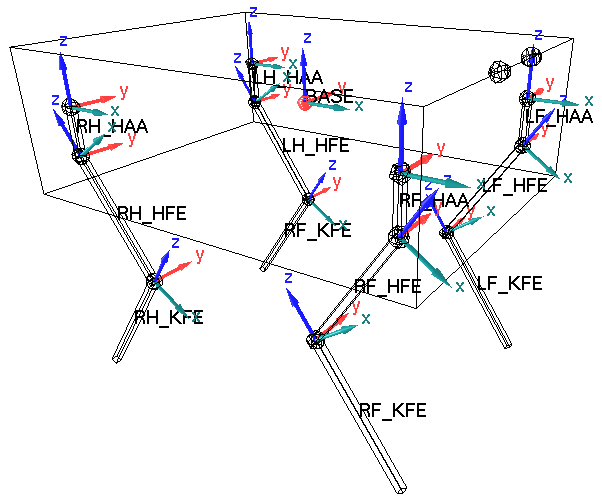
\includegraphics[width=0.4\textwidth]{pics/starleth_frames.png}}	
	\caption{Free floating quadruped Starl\textit{ETH} with a total of 18 DoF.}
	\label{fig:quadruped}
\end{figure}



\lstinputlisting{../../examples/QuadrupedFreeFloat/genEoM.m}


%%%%%%%%%%%%%%%%%%%%%%%%%%%%%%%%%%%%%%%%%%%%%%%%%%%%%%%%%%%%%%%%%%%%%%%%%%%%%%%%%%%%%%%%%%%%%
\clearpage
\section{Generating Code} \label{sec:code}
There are different possibilities to generate code that can be embedded in simulations or controllers:
\begin{itemize}
\item .m function
\item compiled mex functions
\item C-code to embed
\end{itemize}

The matlab script \emph{createFunctionFiles.m} gives you some example code.

\subsection{Generating Matlab Functions and Mex Functions}
% change here the line numbers
%\lstinputlisting[firstline=40, lastline=52]{../../examples/GeneratingCode/createFunctionFiles.m}.
The Symbolic Toolbox of Matlab provides the function \emph{matlabFunction} to generate a matlab function from a symbolic matrix in a m-file:

\begin{lstlisting}
% generate a matlab function
matlabFunction(sys.MpNE,'file','matlabFunc/Mfunc','vars',[sys.q;sys.param]);
matlabFunction(sys.bpNE,'file','matlabFunc/bfunc','vars',[sys.q;sys.dq;sys.param]);
matlabFunction(sys.gpNE,'file','matlabFunc/gfunc','vars',[sys.q;sys.param]);
\end{lstlisting}

The generated files can be used to compile \emph{mex-files} as follows:

\begin{lstlisting}
% compile this matlab function to a mex function
emlc -o mexFunc/Mfunc_mex matlabFunc/Mfunc.m
emlc -o mexFunc/bfunc_mex matlabFunc/bfunc.m
emlc -o mexFunc/gfunc_mex matlabFunc/gfunc.m
\end{lstlisting}

Note: The mex-functions are executed much faster than the matlab-functions for systems with a lot of degrees of freedom.

\subsection{Generating C-Code}
The Symbolic Toolbox of Matlab comes along with the function \emph{ccode} that generates C-code from a symbolic matrix.
The function \emph{ccode} is able to write optimized C-Code in a file. 
Note that the function can also print the code in the command window of Matlab, but that code is not optimized. 


The function \emph{ccode} makes extensive use of auxiliary variables that need to be defined, e.g. as 'const double'.
The following function adds the definitions and re-names the array name:
\lstinputlisting[firstline=1, lastline=13]{../../examples/GeneratingCode/genCCodeMatrix.m}

The function creates a temporary file that could be included somewhere in your code, and outputs the C-code in string.


The Matlab function \emph{genCCodeMatrix} does not add a definition of the array, e.g. 
\begin{lstlisting}
 double MpNE[3][3];
\end{lstlisting}
because the definition might be in another location of your code, e.g. in a class as a member variable.
Moreover, the array needs to be initialized with zero values, because the function \emph{ccode} omits array entries that are zero.


The following Matlab function is an example for generating C-code:
\lstinputlisting[firstline=1, lastline=13]{../../examples/GeneratingCode/genCCodeExampleFile.m}

It creates a simple application that computes the components of the EoM and prints them to the command line.




% \cleardoublepage
% \include{}
% \cleardoublepage
% \include{}
% \cleardoublepage
% ...
%
%---------------------------------------------------------------------------
% Appendix

% \appendix
% \include{appendix}
%
%---------------------------------------------------------------------------
% Literature

% \include{bibliography}
\bibliographystyle{unsrt}
\bibliography{sections/references}

%---------------------------------------------------------------------------

\end{document}
%===========================================================================

